\documentclass[tikz,border=5mm]{standalone}
\usetikzlibrary{calc}
\begin{document}
	%------------------
	\begin{tikzpicture}[scale=2]
		\def\h{3}%chiều cao
		\def\diem(#1)(#2)[#3]{
			\path (#1) coordinate (#2) node[#3] {#2}
			(#2)+(0,\h) coordinate (#21) node[#3] {#21};
		}
		\diem(0,0)(A)[below left]
		\diem(3,0)(B)[below right]
		\diem(1,1.5)(D)[left]
		\diem($(B)+(D)$)(C)[right]
		\draw
		(A1)--(B1)--(C1)--(D1)--(A1)
		(A)--(B)--(C)
		(A)--(A1) (B)--(B1) (C)--(C1);
		\draw[dashed]
		(A)--(D)--(C)
		(D)--(D1);
	\end{tikzpicture}
	%------------------
	
	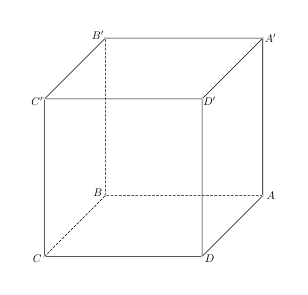
\begin{tikzpicture}[very thin]
		\def\a{2}\def\b{2}\def\c{2}
		\draw[dash pattern=on 1pt off .5pt](\a,0,0)coordinate(A)--(0,0,0)coordinate(B)--(0,0,\c)coordinate(C)(B)--(0,\b,0)coordinate(B');
		\draw(A)--++(B')coordinate(A')--(B')--++(C)coordinate(C')--(C)--++(A)coordinate(D)--(A)(A')--++(C)coordinate(D')--(C')(D')--(D);
		\foreach \p/\g in {A/0,B/160,C/-160,D/-20,A'/0,B'/160,C'/-160,D'/-20}
		\shade[ball color=white](\p)circle(.5pt)node[shift={(\g:.1)},scale=.4]{$\p$};
	\end{tikzpicture}

\begin{tikzpicture}[scale=1,font=\footnotesize]
	\def\a{5}\def\b{4}\def\h{5}
	\path
	(-45:\b) coordinate (C)
	(0,0) coordinate (A)
	(0:\a) coordinate (B)
	%($(A)!0.5!(B)$) coordinate (O)
	($(A)+(C)-(B)$) coordinate (D)
	(90:\h)coordinate (A');
	\foreach \p in {B,C,D}\draw[fill=black] (\p) --($(\p)+(A')$)coordinate (\p');
	\draw[dashed](A)--(B) (A)--(A') (A)--(D);
	\draw (A')--(D')--(C')--(B')--cycle (B)--(C)--(D);
	\foreach \p/\g in {A/150,B/0,C/-90,D/-90,A'/90,D'/90,B'/90,C'/-20}\draw[fill=black] (\p) circle (.7pt)node[shift={(\g:.3)}]{$\p$};
\end{tikzpicture}

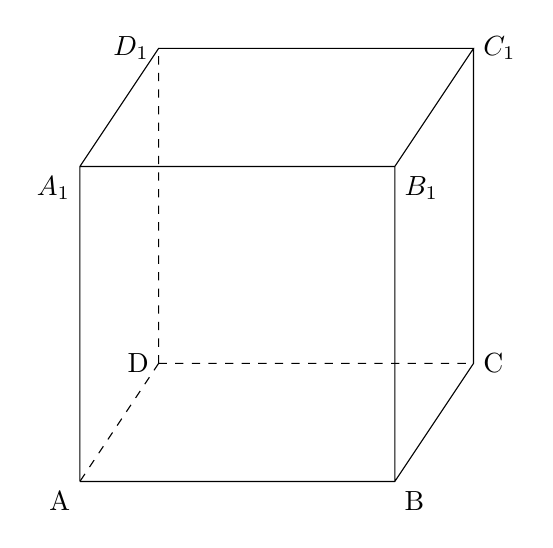
\begin{tikzpicture}
	\def\a{4} %chiều cao
	\path
	(0,0) coordinate (A) node[below left] {A}
	(\a,0) coordinate (B) node[below right] {B}
	(1,1.5) coordinate (D) node[left] {D}
	(D)+(\a,0) coordinate (C) node[right] {C}
	(A)+(0,\a) coordinate (A1) node[below left] {$A_1$}
	(B)+(0,\a) coordinate (B1) node[below right] {$B_1$}
	(D)+(0,\a) coordinate (D1) node[left] {$D_1$}
	(C)+(0,\a) coordinate (C1) node[right] {$C_1$};
	\draw[dashed] (D)--(A) (D)--(C) (D)--(D1);
	\draw
	(A1)--(B1)--(C1)--(D1)--(A1)
	(A)--(B)--(C)
	(A)--(A1) (B)--(B1) (C)--(C1);
\end{tikzpicture}

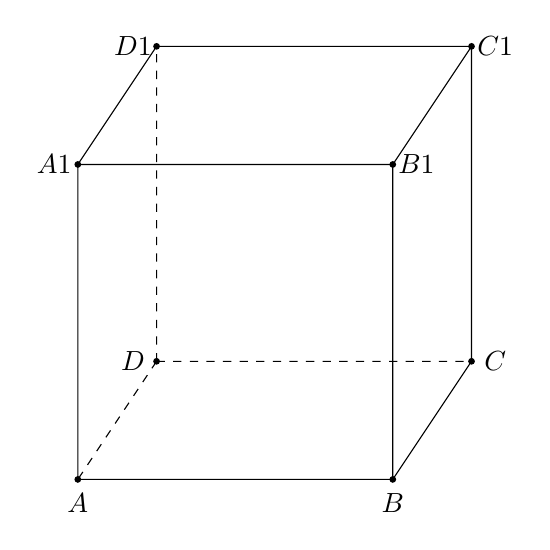
\begin{tikzpicture}
	\def\a{4} %chiều cao
	\path
	(0,0) coordinate (A)
	(\a,0) coordinate (B)
	(1,1.5) coordinate (D)
	(D)+(\a,0) coordinate (C);
	\foreach \x in {A,B,C,D}
	\path (\x)+(0,\a) coordinate(\x1);
	\draw[dashed] (D)--(A) (D)--(C) (D)--(D1);
	\draw
	(A1)--(B1)--(C1)--(D1)--(A1)
	(A)--(B)--(C)
	(A)--(A1) (B)--(B1) (C)--(C1);
	\foreach \p/\g in {A/-90,B/-90,C/0,D/180,A1/180,B1/0,C1/0,D1/180}\draw[fill=black] (\p) circle (1pt)node[shift={(\g:.3)}]{$\p$};
\end{tikzpicture}
\end{document}